%
% file: localoperator.tex
% author: Victor Brena
% description: Briefly describes properties of the local operator.
%

\chapter{Appendix A}
\label{app:app01}

\section{Risk Matrix}

\begin{figure}[H]
	\centering
	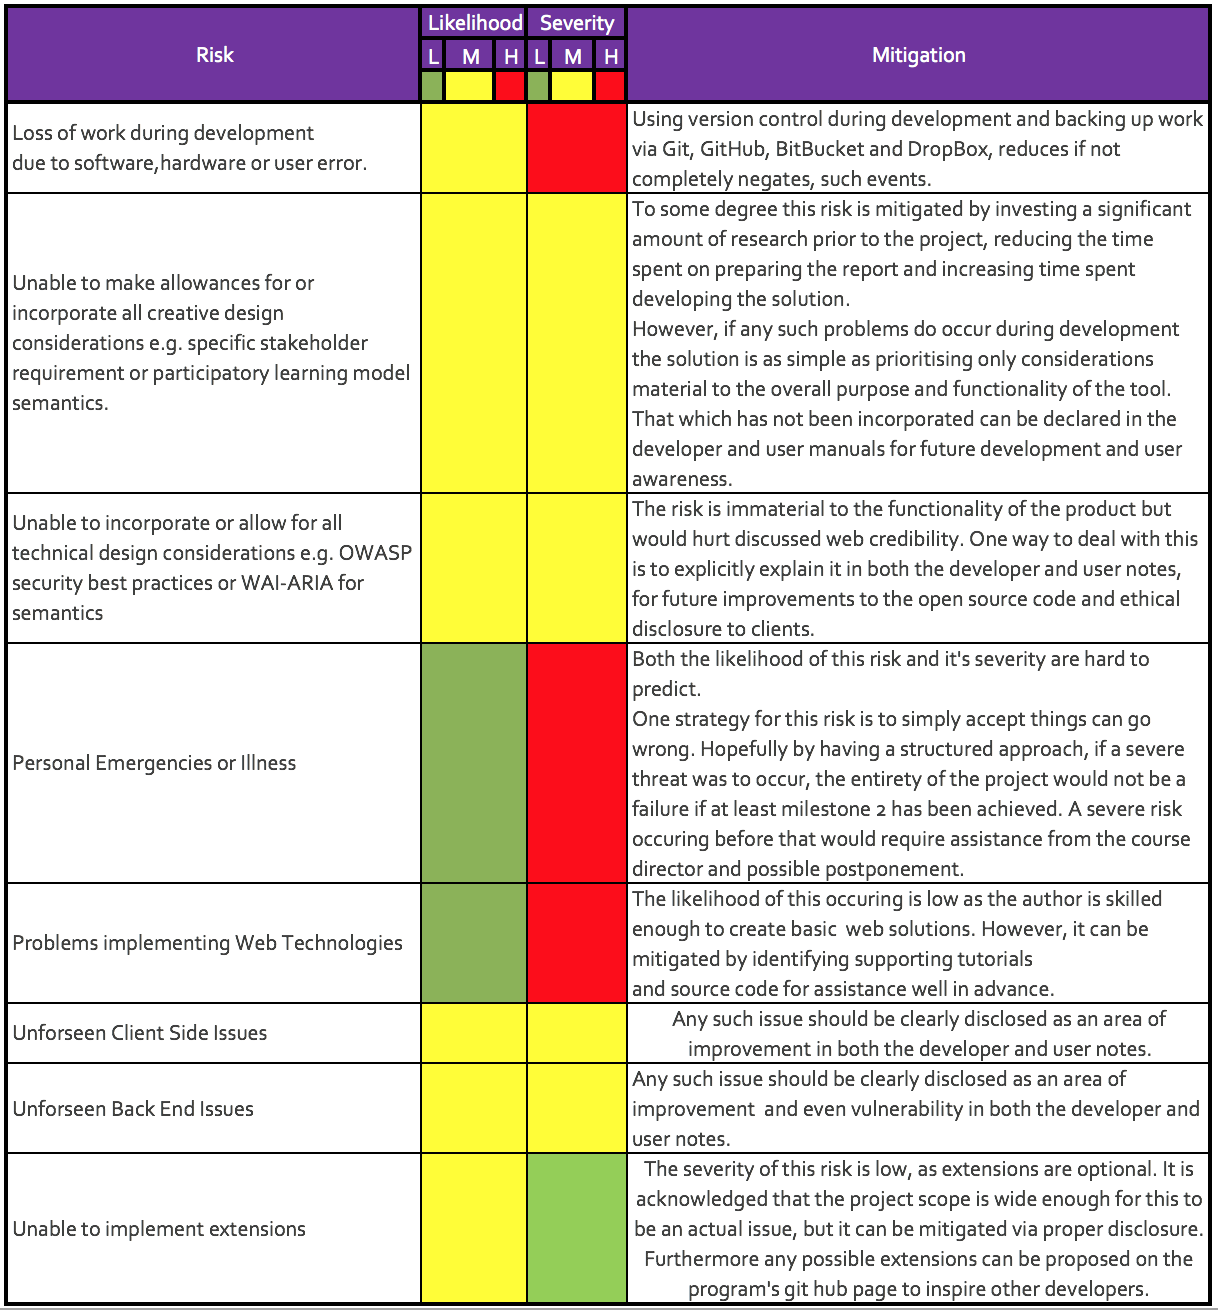
\includegraphics[scale=.68]{figures/risk}
	\mycaption[Risk Matrix]{Risk Matrix}
	\label{fig:Risk Matrix}
\end{figure}
\newpage

\section{Project Milestones, Tasks and Resultant List of Deliverables}
\begin{figure}[H]
	\centering
	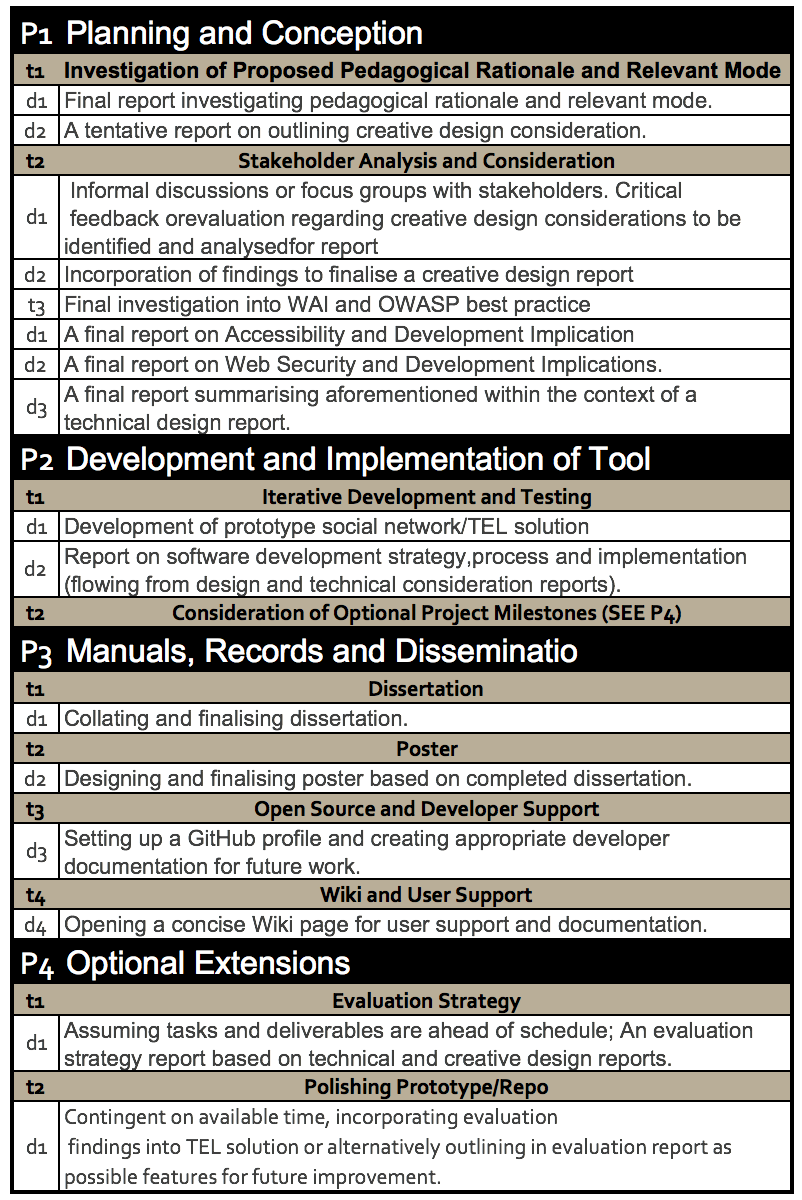
\includegraphics[scale=.9]{figures/summary}
	\mycaption[List of Deliverables, Milestones and Tasks]{List of Deliverables, Milestones and Tasks.}
	\label{fig:List of Deliverables, Milestones and Tasks}
\end{figure}


\section{Gantt Chart}
\begin{figure}[H]
	\centering
	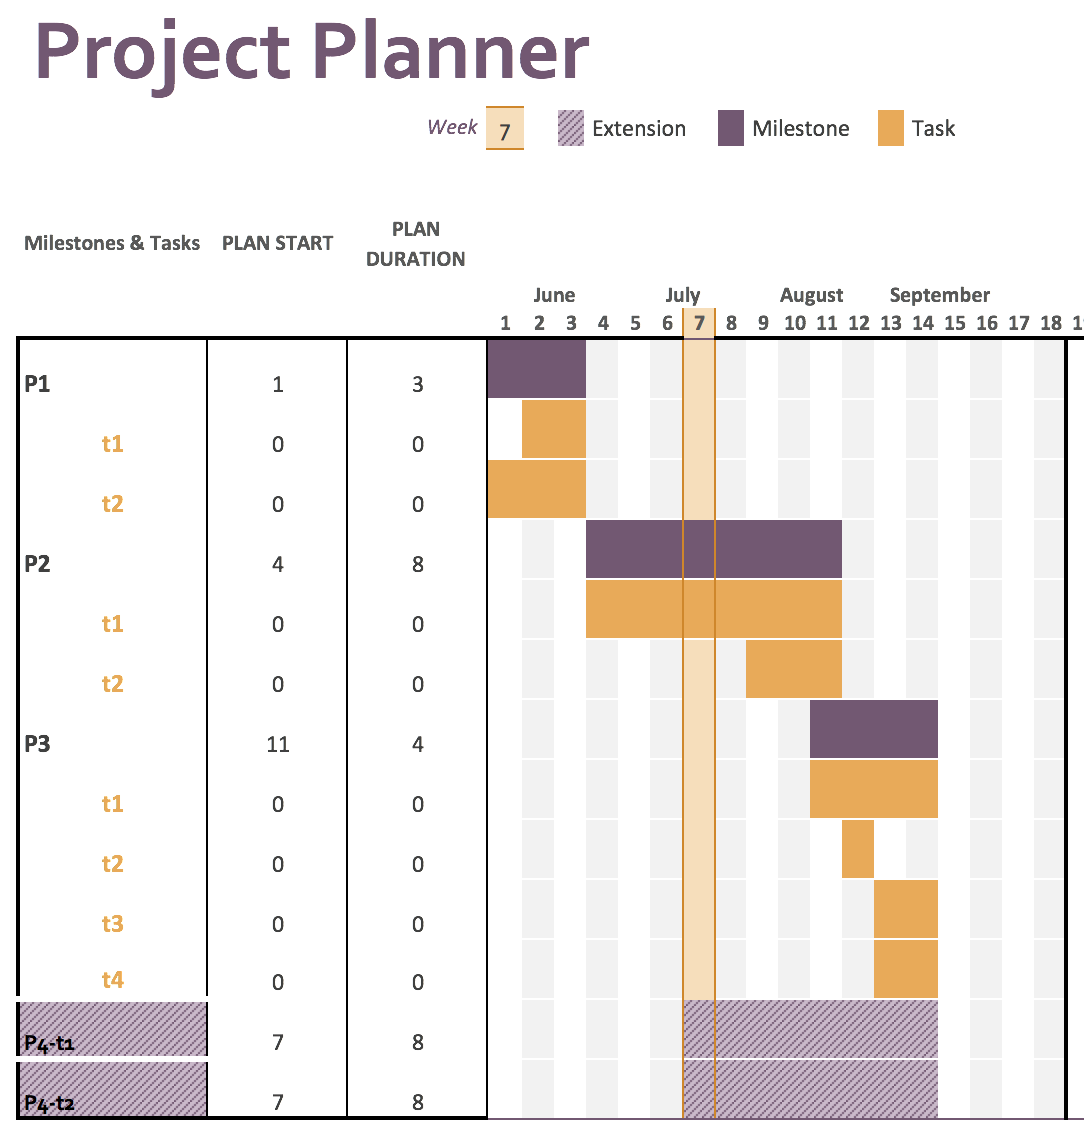
\includegraphics[scale=.75]{figures/Gantt}
	\mycaption[Project Planner: Gantt Chart]{Project Planner: Gantt Chart.}
	\label{fig:Gantt}
\end{figure}